\chapter{文獻回顧}

\section{插入圖片範例}

我是有肉,我是有肉,我是有肉,我是有肉,我是有肉,我是有肉,我是有肉,我是有肉,我是有肉,我是有肉,我是有肉,我是有肉,我是有肉,我是有肉,我是有肉,我是有肉,我是有肉,我是有肉,我是有肉,我是有肉,我是有肉,我是有肉,我是有肉,我是有肉,我是有肉,我是有肉,我是有肉,我是有肉,我是有肉,我是有肉,我是有肉,我是有肉,我是有肉,我是有肉。%%%之後若需加入新圖片僅需依照本檔案格式來創建即可,在本文中插入圖片的方式可參考chapters中文獻回顧檔案的範例。

%-------------------------------------------------------------


\begin{figure}[!htbp]

\centering


%上傳完成後至此資料夾創建一個新的檔案
%下面這行的最後一個{}加入image 中的圖片路徑
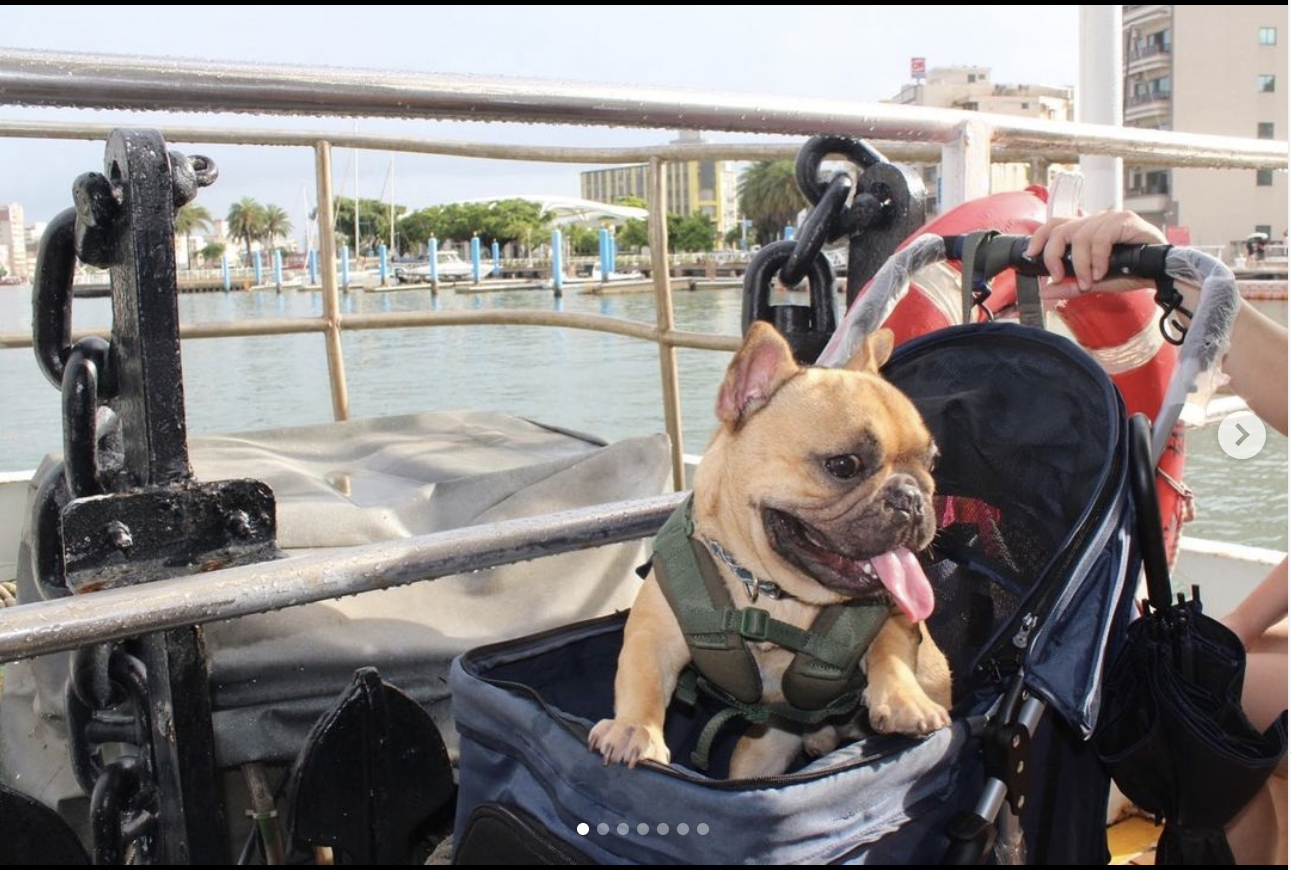
\includegraphics[width=1\textwidth]{images/yolo.png}

%下面這行書入圖片標題即可
\caption{有肉可愛}



\label{i:flow chart}
\end{figure}




我是有肉,我是有肉,我是有肉,我是有肉,我是有肉,我是有肉,我是有肉,我是有肉,我是有肉,我是有肉,我是有肉,我是有肉,我是有肉,我是有肉,我是有肉,我是有肉,我是有肉,我是有肉,我是有肉,我是有肉,我是有肉,我是有肉,我是有肉,我是有肉,我是有肉,我是有肉,我是有肉,我是有肉,我是有肉,我是有肉,我是有肉,我是有肉,我是有肉,我是有肉,我是有肉。/par



%%如上只需使用\input{圖片路徑}即可插入圖片。
%%所插入的圖片會自動依照章節編入圖目錄中,無需再進行更動。















































